\chapter{Patent and Proprietary Stamps} 

\begin{marginfigure}
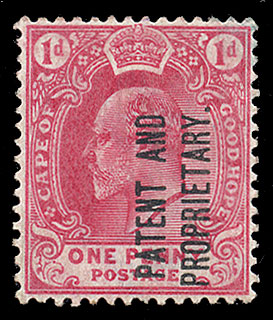
\includegraphics[width=1.0\textwidth]{../cape-of-good-hope/revenue-patent.jpg}

\caption{1909 KEVII 1d carmine overprinted PATENT AND PROPRIETARY. in black reading vertically upward. SG 71 var. The stamp was overprinted due to rate changes in 1909.}

\end{marginfigure}
In 1908 and new form of taxation was introduced in the Cape of Good Hope. By means of stamp duties all medicine was to be taxed. Brian Trotter<sup>1</sup> gives the reason that the tax was introduced so that additional revenue could be earned as the coming up of the National Convention to discuss the Union of the South Africa, the Cape's prime Minister feared that the Cape's influence would be diminihed at the convention if the financial position was not strengthened.

Initially the stamps were produced locally, probably by the Cape Times. the values of these stamps were 2d, 4d, 6d, 2s 6d, 4s 6d, 10s and \pound1. The stamp ws designed by Sturman, Chief Clerk of the Government Post office and the designed selected by the Cape prime Minister, John Merriman, as the most suitable from the six designs submitted by Sturman. These stamps were the only locally printed stamps during the Edwardian Period.

No convincing reason can be found as why existing revenue stamps could not have been used for this purpose, or at least overprinting them.




The Act No.39 of September, 1908 prescribed that the duty was to be collected by
"means of stamps".

\begin{verbatim}
Medicine Price     Stamp Duty
Retail (up to)
1s6d				2d
2s6d				4d
  4s				6d
 10s 			  1s6d	
\pound1           2s6d 
\pound1 10s       4s6d
\pound2 10s        10s
Over \pound2 10s  \pound1
\end{verbatim}

The Act had only been in place for a little more than a year, when an amendement was issued
by Act No.16 of 30 november 1909. This changed the duty on patent and proprietary medicines to 2d if the container retailed at less than 1s6d, then an "additional stamp duty of 1d for every additional 6d or part thereof of such price".

This change in the regulations impacted on the stmps required, as it now required the
issue of a 1d stamp. Ths denomination was not avialble either at the local printing or De La Rue. To alleviate the problem the then current 1d Cape postage stamps, were overprinted.

The stamps were required to be affixed to the box, bottles and other containers holding the medicines, they were discarded with the empty containers and very few
have survived used.

This duty was repelled by the South Africa Act No. 30 of 1 July 1911.

\ph[width = .80\textwidth]{../cape-of-good-hope/patent-01.jpg}{De La Rue's First design proposal.}


\subsubsection{References}

1. Trotter Brian, Cape of Good Hope Patent and Proprietary Stamps, \textit{London Philatelist}, March 2002, \textbf{111}:57. 
2. Government Gazettes and Acts of Parliament of the Cape of Good Hope and the Union of South Africa.            